\section{Interpretasi Hasil Simulasi qPCA}

\begin{frame}{Akumulasi Probabilitas pada Spektral QPhE}
    \begin{columns}
        \begin{column}{0.5\textwidth}
            \begin{itemize}
                \item Gambar di samping mengilustrasikan dominasi fasa akibat interferensi konstruktif masif yang mengisolasi amplitudo secara mutlak pada keadaan biner $|111\rangle$.
                \item Terminologi representasi biner kuantum tersebut secara matematis merepresentasikan nilai probabilitas desimal numerik $\Lambda \approx 0.875$.
                \item Distribusi empiris ini mematuhi prediksi resolusi ortogonal hasil komputasi dekomposisi klasik yang mencatat titik kritis \textit{eigenvalue} utama pada $\lambda_1 = 0.8576$.
            \end{itemize}
        \end{column}
        \begin{column}{0.5\textwidth}
            \begin{figure}
                \centering
                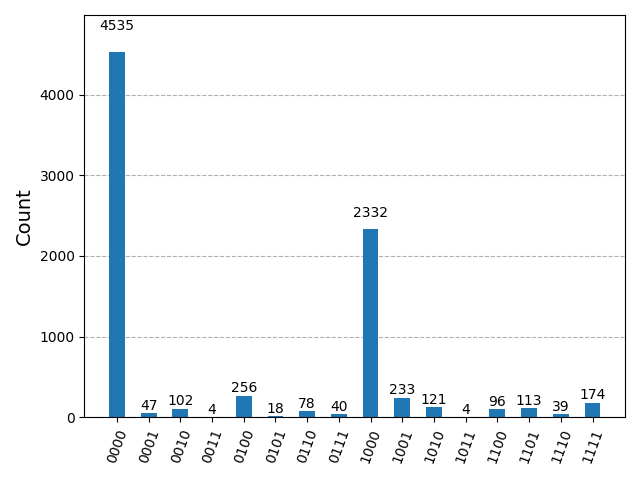
\includegraphics[width=\textwidth,keepaspectratio]{QPCA-master/qpca_qphe_result.png}
                \caption{Ekspektasi observasi keluaran dari modul QPhE.}
            \end{figure}
        \end{column}
    \end{columns}
\end{frame}

\begin{frame}{Evaluasi Kemurnian State Kuantum dan Rotasi Vektor Bloch}
    \begin{columns}
        \begin{column}{0.5\textwidth}
            \begin{figure}
                \centering
                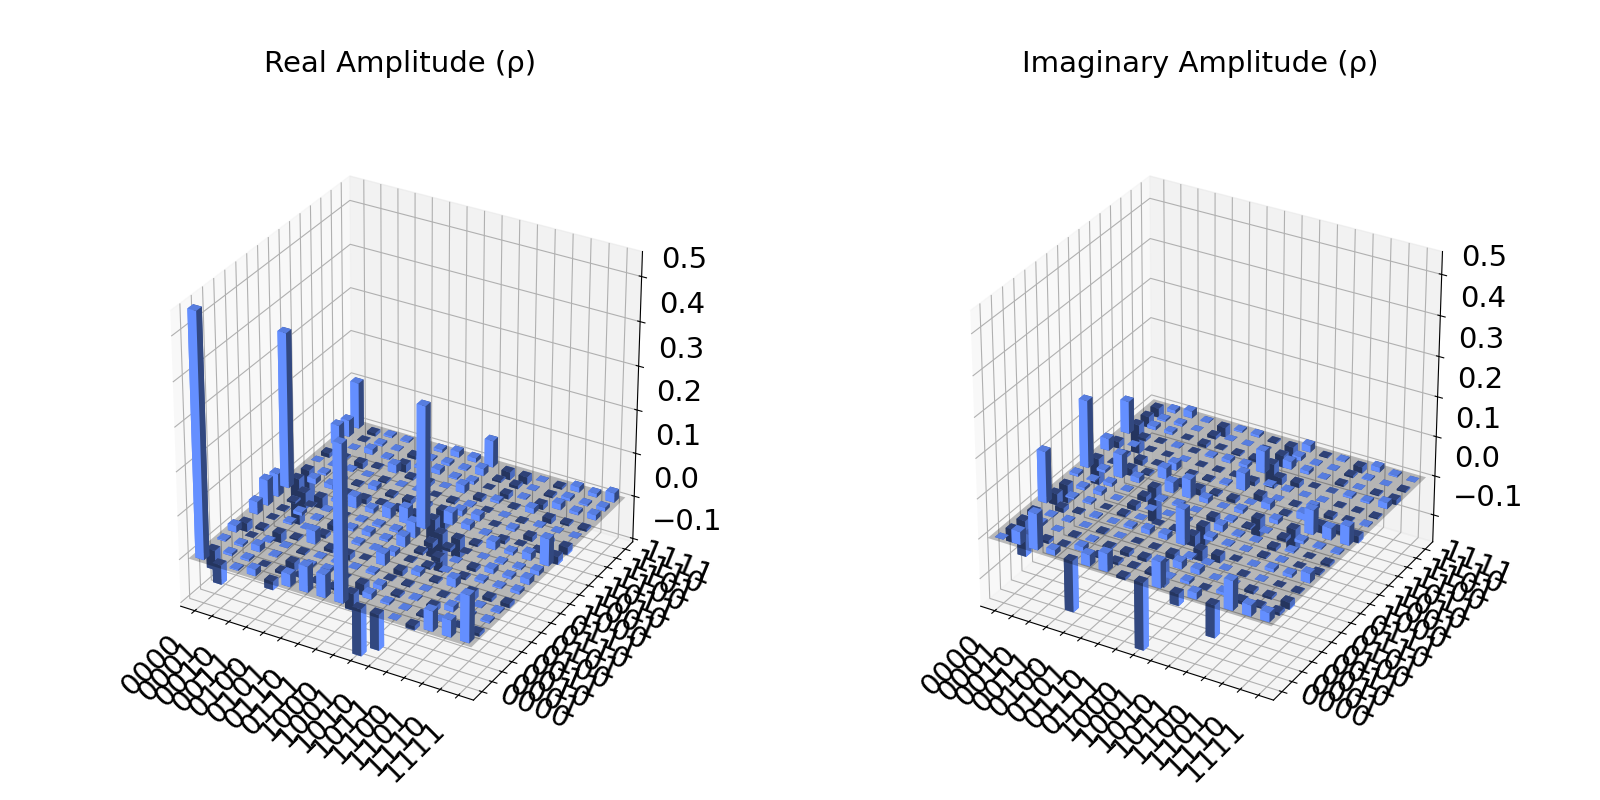
\includegraphics[width=0.8\textwidth,keepaspectratio]{QPCA-master/state_city_qphe.png}
                \caption{Densitas visibilitas \textit{state city} QPhE.}
            \end{figure}
        \end{column}
        \begin{column}{0.5\textwidth}
            \begin{figure}
                \centering
                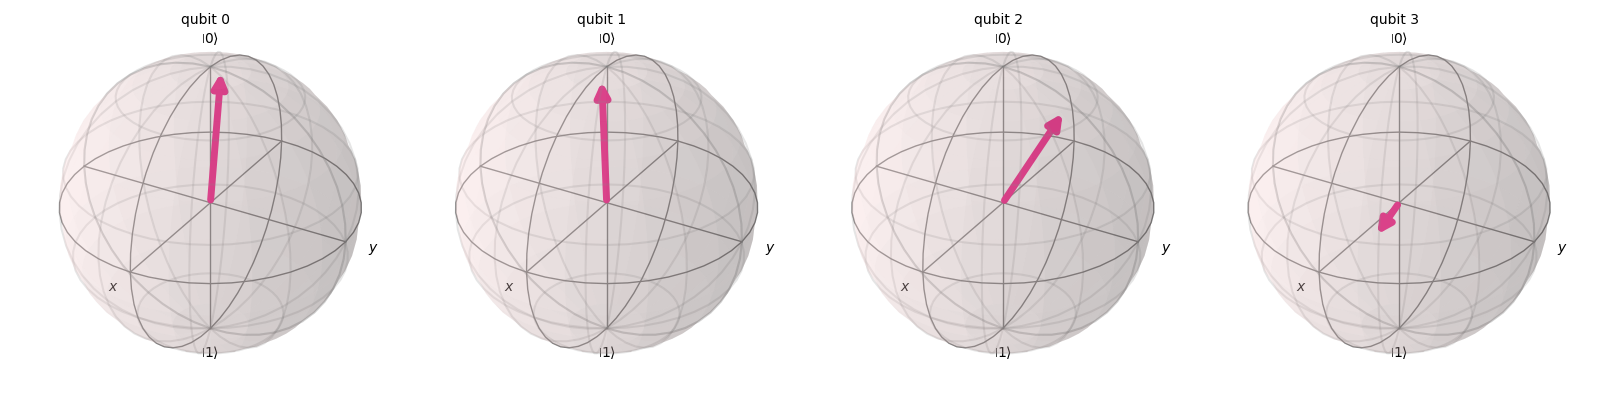
\includegraphics[width=0.8\textwidth,keepaspectratio]{QPCA-master/bloch_qphe.png}
                \caption{Rotasi geometris pada bola Bloch murni.}
            \end{figure}
        \end{column}
    \end{columns}
    \begin{itemize}
        \item Eksplorasi grafis matriks \textit{state city} dan rotasi bola Bloch mengonfirmasi terpeliharanya densitas kemurnian uniter. Sistem bertahan utuh tanpa reduksi fasa yang memicu hilangnya memori kuantum (\textit{spontaneous relaxation}).
    \end{itemize}
\end{frame}

\begin{frame}{Stabilitas Validasi \textit{Eigenstate}: Resistansi Terhadap Ekstrapolasi Noise}
    \begin{columns}
        \begin{column}{0.5\textwidth}
            \begin{itemize}
                \item Gambar di samping merepresentasikan superioritas rasio \textit{signal-to-noise} (\textit{SNR}), yang mengindikasikan bahwa peredaman fasa parasit oleh interferensi destruktif berjalan sempurna.
                \item Fenomena konvergensi fasa menjadi justifikasi rasionalitas bahwa deret parameter rotasi kuantum internal divalidasi memiliki koherensi tinggi serta memiliki daya presisi analitik yang kuat.
            \end{itemize}
        \end{column}
        \begin{column}{0.5\textwidth}
            \begin{figure}
                \centering
                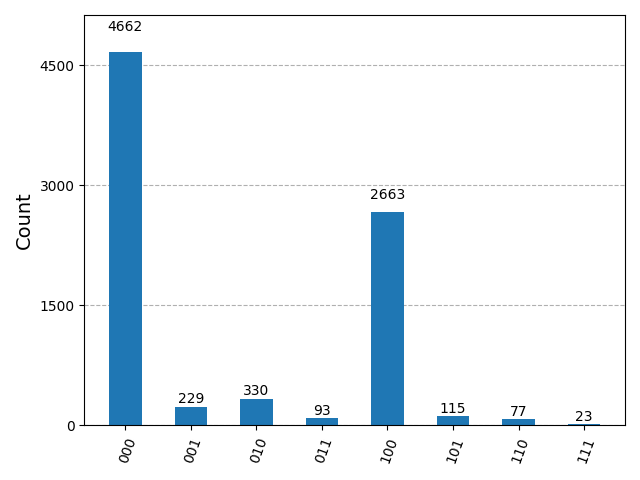
\includegraphics[width=\textwidth,keepaspectratio]{QPCA-master/qpca_eigenstate_result.png}
                \caption{Konsistensi frekuensi stabil state interferensi destruktif.}
            \end{figure}
        \end{column}
    \end{columns}
\end{frame}

\begin{frame}{Erosi Koherensi pada Beban Dimensional Tinggi ($4 \times 4$)}
    \begin{columns}
        \begin{column}{0.5\textwidth}
            \begin{itemize}
                \item Gambar di samping memvisualisasikan disipasi informasi ekstrem; distribusi pengukuran kuantum berubah menjadi profil seragam (\textit{uniform}) sebagai simptom dekoherensi absolut.
                \item Eksplosi persentase galat per-gerbang 2-qubit menjamur hingga total $> 100\%$, menciptakan batasan operasional absolut bagi kemampuan mesin iterasi eksperimental era NISQ.
                \item Insiden empiris tersebut mendeklarasikan bahwa manipulasi sistem finansial \textit{hybrid} wajib didukung secara radikal oleh instrumen ekstrapolasi mitigasi canggih seperti \textit{Richardson’s error mitigation}.
            \end{itemize}
        \end{column}
        \begin{column}{0.5\textwidth}
            \begin{figure}
                \centering
                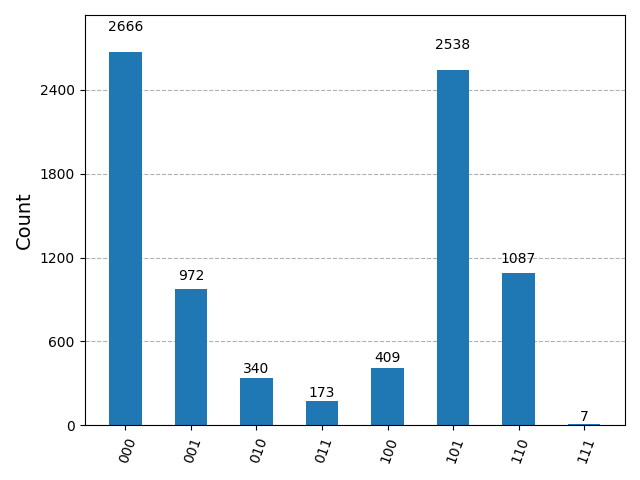
\includegraphics[width=\textwidth,keepaspectratio]{QPCA-master/qpca_4x4_result.png}
                \caption{Disipasi fasa absolut pada skenario uji densitas $4 \times 4$.}
            \end{figure}
        \end{column}
    \end{columns}
\end{frame}

\begin{frame}{Manifestasi Kekaburan Matriks \textit{Off-Diagonal} pada Tomografi $4 \times 4$}
    \begin{columns}
        \begin{column}{0.5\textwidth}
            \begin{figure}
                \centering
                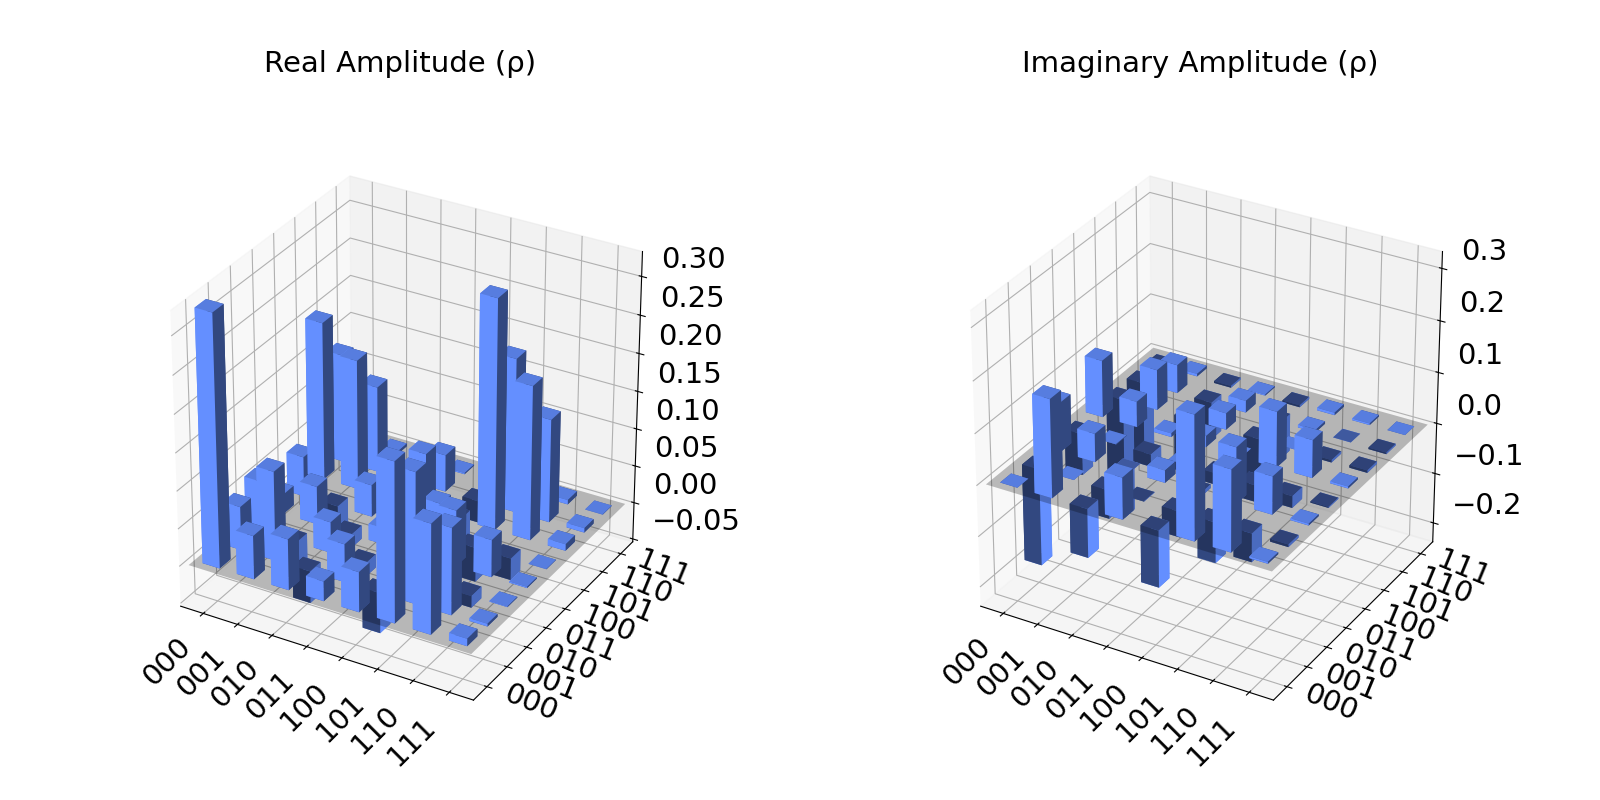
\includegraphics[width=\textwidth,keepaspectratio]{QPCA-master/state_city_4x4.png}
            \end{figure}
        \end{column}
        \begin{column}{0.5\textwidth}
            \begin{figure}
                \centering
                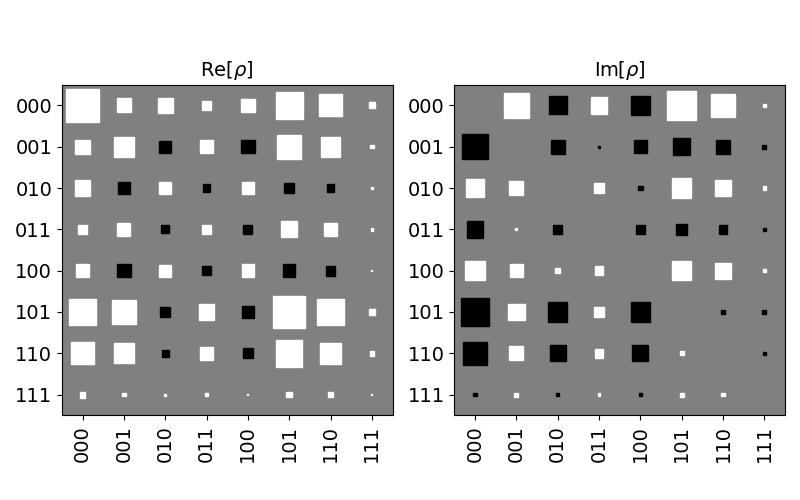
\includegraphics[width=\textwidth,keepaspectratio]{QPCA-master/hinton_4x4.png}
            \end{figure}
        \end{column}
    \end{columns}
    \begin{itemize}
        \item Representasi topografi \textit{state city} (kiri) bersama dengan grafis peta \textit{Hinton} (kanan) memanifestasikan insiden bercampurnya spektral komponen \textit{off-diagonal} sekunder secara dominan.
        \item Dinamika ini mempreteli atribut ortogonalitas intrinsik dan memberikan legitimasi mengenai kesulitan matematis dalam memecahkan model kompleks tanpa proteksi galat komprehensif.
    \end{itemize}
\end{frame}
